% Copyright 2006 by Till Tantau
%
% This file may be distributed and/or modified
%
% 1. under the LaTeX Project Public License and/or
% 2. under the GNU Free Documentation License.
%
% See the file doc/generic/pgf/licenses/LICENSE for more details.


\section{Background Library}
\label{section-tikz-backgrounds}

\begin{tikzlibrary}{backgrounds}
    This library defines ``backgrounds'' for pictures. This does not refer to
    background pictures, but rather to frames drawn around and behind pictures.
    For example, this package allows you to just add the |framed| option to a
    picture to get a rectangular box around your picture or |gridded| to put a
    grid behind your picture.
\end{tikzlibrary}
%
\begin{codeexample}[setup code,hidden]
    \usetikzlibrary{backgrounds}
\end{codeexample}

The first use of this library is to make the following key available:
%
\begin{key}{/tikz/on background layer=\meta{options}}
    This key can (only) be used with a |{scope}| or |\scoped|. It will cause
    everything inside the scope to be typeset on a background layer.

    The \meta{options} will be executed \emph{inside} background scope. This is
    useful since \emph{other} options passed to the |{scope}| environment will
    be executed \emph{before} the actual background material starts and, thus,
    will have no effect on it.
    %
\begin{codeexample}[]

\begin{tikzpicture}
  % On main layer:
  \fill[blue] (0,0) circle (1cm);

  \begin{scope}[on background layer={color=yellow}]
    \fill (-1,-1) rectangle (1,1);
  \end{scope}

  \begin{scope}[on background layer]
    \fill[black] (-.8,-.8) rectangle (.8,.8);
  \end{scope}

  % On main layer again:
  \fill[blue!50] (-.5,-1) rectangle (.5,1);
\end{tikzpicture}
\end{codeexample}

    A scope with this option set should not be ``deeply nested'' inside the
    picture since changes to the graphic state (like the color or the
    transformation matrix) ``do not survive a layer switch'', see also
    Section~\ref{section-layers} for details. In particular, setting, say, the
    line width at the beginning of a picture will not have an effect on the
    background picture.

    For this reason, it may be useful to setup the following style:
    %
    \begin{stylekey}{/tikz/every on background layer}
        This style is executed at the beginning of each background layer. If
        you have a global setup in |every picture|, you should consider putting
        that part of it that concerns the graphics state into this style.
        %
\begin{codeexample}[]
\tikzset{
  every picture/.style={line width=1ex},
  every on background layer/.style={every picture}
}
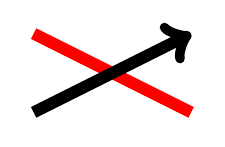
\begin{tikzpicture}
  \draw [->] (0,0) -- (2,1);

  \scoped[on background layer]
    \draw[red] (0,1) -- (2,0);
\end{tikzpicture}
\end{codeexample}
    \end{stylekey}
\end{key}

When this package is loaded, the following styles become available:
%
\begin{stylekey}{/tikz/show background rectangle}
    This style causes a rectangle to be drawn behind your graphic. This style
    option must be given to the |{tikzpicture}| environment or to the |\tikz|
    command.
    %
\begin{codeexample}[]
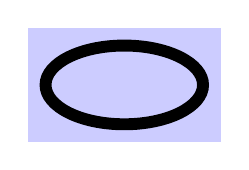
\begin{tikzpicture}[show background rectangle]
  \draw (0,0) ellipse (10mm and 5mm);
\end{tikzpicture}
\end{codeexample}
    %
    The size of the background rectangle is determined as follows: We start
    with the bounding box of the picture. Then, a certain separator distance is
    added on the sides. This distance can be different for the $x$- and
    $y$-directions and can be set using the following options:
    %
    \begin{key}{/tikz/inner frame xsep=\meta{dimension} (initially 1ex)}
        Sets the additional horizontal separator distance for the background
        rectangle.
    \end{key}
    %
    \begin{key}{/tikz/inner frame ysep=\meta{dimension} (initially 1ex)}
        Same for the vertical separator distance.
    \end{key}
    %
    \begin{key}{/tikz/inner frame sep=\meta{dimension}}
        Sets the horizontal and vertical separator distances simultaneously.
    \end{key}
    %
    The following two styles make setting the inner separator a bit easier to
    remember:
    %
    \begin{stylekey}{/tikz/tight background}
        Sets the inner frame separator to 0pt. The background rectangle will
        have the size of the bounding box.
    \end{stylekey}
    %
    \begin{stylekey}{/tikz/loose background}
        Sets the inner frame separator to 2ex.
    \end{stylekey}

    You can influence how the background rectangle is rendered by setting the
    following style:
    %
    \begin{stylekey}{/tikz/background rectangle (initially draw)}
        This style dictates how the background rectangle is drawn or filled.
        The default setting causes the path of the background rectangle to be
        drawn in the usual way. Setting this style to, say, |fill=blue!20|
        causes a light blue background to be added to the picture. You can also
        use more fancy settings as shown in the following example:
        %
\begin{codeexample}[]
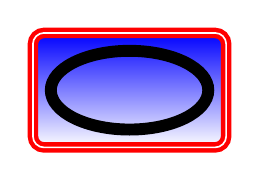
\begin{tikzpicture}
  [background rectangle/.style=
     {double,ultra thick,draw=red,top color=blue,rounded corners},
   show background rectangle]
  \draw (0,0) ellipse (10mm and 5mm);
\end{tikzpicture}
\end{codeexample}
        %
        Naturally, no one in their right mind would use the above, but here is
        a nice background:
        %
\begin{codeexample}[]
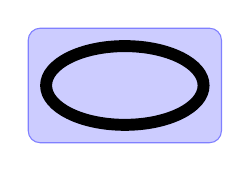
\begin{tikzpicture}
  [background rectangle/.style=
     {draw=blue!50,fill=blue!20,rounded corners=1ex},
   show background rectangle]
  \draw (0,0) ellipse (10mm and 5mm);
\end{tikzpicture}
\end{codeexample}
    \end{stylekey}
\end{stylekey}

\begin{stylekey}{/tikz/framed}
    This is a shorthand for |show background rectangle|.
\end{stylekey}

\begin{stylekey}{/tikz/show background grid}
    This style behaves similarly to the |show background rectangle| style, but
    it will not use a rectangle path, but a grid. The lower left and upper
    right corner of the grid is computed in the same way as for the background
    rectangle:
    %
\begin{codeexample}[]
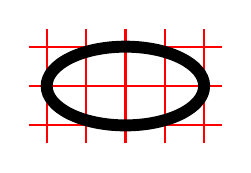
\begin{tikzpicture}[show background grid]
  \draw (0,0) ellipse (10mm and 5mm);
\end{tikzpicture}
\end{codeexample}
    %
    You can influence the background grid by setting the following style:
    %
    \begin{stylekey}{/tikz/background grid (initially draw,help lines)}
        This style dictates how the background grid path is drawn.
        %
\begin{codeexample}[]
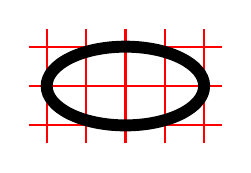
\begin{tikzpicture}
  [background grid/.style={thick,draw=red,step=.5cm},
   show background grid]
  \draw (0,0) ellipse (10mm and 5mm);
\end{tikzpicture}
\end{codeexample}
    \end{stylekey}
    %
    This option can be combined with the |framed| option (use the |framed|
    option first):
    %
\begin{codeexample}[]
\tikzset{background grid/.style={thick,draw=red,step=.5cm},
         background rectangle/.style={rounded corners,fill=yellow}}
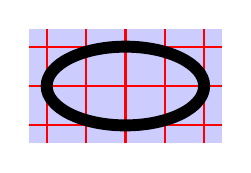
\begin{tikzpicture}[framed,gridded]
  \draw (0,0) ellipse (10mm and 5mm);
\end{tikzpicture}
\end{codeexample}
    %
\end{stylekey}

\begin{stylekey}{/tikz/gridded}
    This is a shorthand for |show background grid|.
\end{stylekey}

\begin{stylekey}{/tikz/show background top}
    This style causes a single line to be drawn at the top of the background
    rectangle. Normally, the line coincides exactly with the top line of the
    background rectangle:
    %
\begin{codeexample}[]
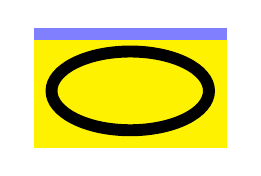
\begin{tikzpicture}[
    background rectangle/.style={fill=yellow},
    framed,show background top]
  \draw (0,0) ellipse (10mm and 5mm);
\end{tikzpicture}
\end{codeexample}
    %
    The following option allows you to lengthen (or shorten) the line:
    %
    \begin{key}{/tikz/outer frame xsep=\meta{dimension} (initially 0pt)}
        The \meta{dimension} is added at the left and right side of the line.
        %
\begin{codeexample}[]
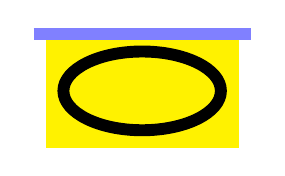
\begin{tikzpicture}
  [background rectangle/.style={fill=yellow},
   framed,
   show background top,
   outer frame xsep=1ex]
  \draw (0,0) ellipse (10mm and 5mm);
\end{tikzpicture}
\end{codeexample}
    \end{key}
    %
    \begin{key}{/tikz/outer frame ysep=\meta{dimension} (initially 0pt)}
        This option does not apply to the top line, but to the left and right
        lines, see below.
    \end{key}
    %
    \begin{key}{/tikz/outer frame sep=\meta{dimension}}
        Sets both the $x$- and $y$-separation.
    \end{key}
    %
\begin{codeexample}[]
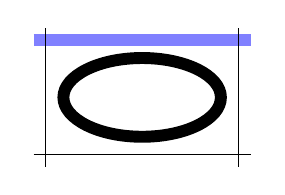
\begin{tikzpicture}
  [background rectangle={fill=blue!20},
   outer frame sep=1ex,%
   show background top,%
   show background bottom,%
   show background left,%
   show background right]
  \draw (0,0) ellipse (10mm and 5mm);
\end{tikzpicture}
\end{codeexample}
    %
    You can influence how the line is drawn grid by setting the following
    style:
    %
    \begin{stylekey}{/tikz/background top (initially draw)}
\begin{codeexample}[]
\tikzset{background rectangle/.style={fill=blue!20},
         background top/.style={draw=blue!50,line width=1ex}}
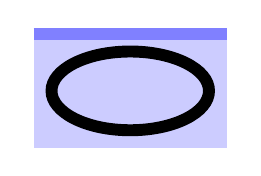
\begin{tikzpicture}[framed,show background top]
  \draw (0,0) ellipse (10mm and 5mm);
\end{tikzpicture}
\end{codeexample}
    \end{stylekey}
\end{stylekey}

\begin{stylekey}{/tikz/show background bottom}
    Works like the style for the top line.
\end{stylekey}

\begin{stylekey}{/tikz/show background left}
    Works similarly.
\end{stylekey}

\begin{stylekey}{/tikz/show background right}
    Works similarly.
\end{stylekey}


%%% Local Variables:
%%% mode: latex
%%% TeX-master: "pgfmanual-pdftex-version"
%%% End:
